\chapter{TF2}

\section{Définition}

\textit{tf2} est une bibliothèque de ROS2 permettant de gérer plusieurs repères de coordonnées en parallèle. Cela est particulièrement utile lorsque différents composants d'un système utilisent chacun leur propre repère. Par exemple, un système de Motion Capture fournit la position d'un robot dans un repère global fixe, tandis que chaque robot dispose de son propre repère local, centré sur lui-même. Se déplacer selon l'axe $x$ du repère de Motion Capture ne correspond donc pas nécessairement à un mouvement vers l'avant pour le robot. 

\begin{figure}[H]
    \centering
    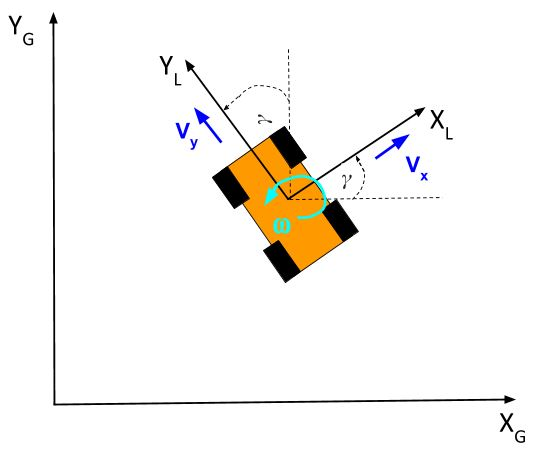
\includegraphics[width=0.6\textwidth]{Annexes/Mecanum_ROS2/tf2/pictures/frame_coordinate.jpg}
    \caption{Repère globale et repère Body}
    \label{fig:multiple_frame}
\end{figure}

Prenons l'exemple Figure \ref{fig:multiple_frame}, le robot est piloté par des commandes de vitesses linéaires exprimées dans son repère local $X_L,Y_L$. Si une commande de vitesse $v_x > 0$ est envoyée, le robot avancera dans la direction de son axe $X_L$, quelle que soit son orientation dans le repère global. Toutefois, si tous les calculs (planification, contrôle en formation, navigation, etc.) sont effectués dans le repère global $X_G, Y_G$, il est alors nécessaire de transformer ces vitesses depuis le repère global vers le repère local du robot avant de les lui envoyer. Inversement, les positions ou vitesses mesurées dans le repère local doivent être transformées dans le repère global pour être comparées ou utilisées dans les algorithmes centraux. 

\textit{tf2} permet donc de convertir les positions, orientations ou vitesses d'un repère à un autre, ce qui permet de piloter ou d'observer le robot dans le repère qui est le plus pertinent pour la tâche à accomplir.

\newpage
\section{Mise en place de tf2 }

\subsection{Initialisation de tf2 : Buffer, Listener et Broadcaster}

\noindent Dans un premier temps, il faut initialiser trois composants principaux :
\begin{itemize}
    \item \textbf{Buffer} : stocke les transformations entre repères.
    \item \textbf{TransformListener} : écoute les transformations publiées sur le réseau ROS et alimente le buffer.
    \item \textbf{TransformBroadcaaaster} : permet de publier de nouvelles transformations (par exemple, la position du robot dans le repère global).
\end{itemize}
\vspace{0.1cm}

\begin{lstlisting}[style=commandstyle, caption={Initialisation de tf2 dans un nœud ROS2}]
from tf2_ros import Buffer, TransformListener, TransformBroadcaster

class MyNode(Node):
    def __init__(self):
        super().__init__('my_tf2_node')
        self.tf_buffer = Buffer()
        self.tf_listener = TransformListener(self.tf_buffer, self)
        self.tf_broadcaster = TransformBroadcaster(self)
\end{lstlisting}

\subsection{Publication de la transformation du robot}

À chaque réception d'une nouvelle pose (par exemple depuis un système de Motion Capture), il faut publier la transformation entre le repère global (ex: \textit{mocap}) et le repère du robot (ex: \textit{robot\_name/base\_link}). 
\hspace{0.2cm}
\begin{lstlisting}[style=commandstyle, caption={Publication de la transformation à partir de la pose}]
from geometry_msgs.msg import TransformStamped

def pose_callback(self, msg):
    transform = TransformStamped()
    transform.header.stamp = self.get_clock().now().to_msg()
    transform.header.frame_id = "mocap"  # repere global
    transform.child_frame_id = "robot_name/base_link"  # repere du robot

    transform.transform.translation.x = msg.pose.position.x
    transform.transform.translation.y = msg.pose.position.y
    transform.transform.translation.z = msg.pose.position.z

    transform.transform.rotation.x = msg.pose.orientation.x
    transform.transform.rotation.y = msg.pose.orientation.y
    transform.transform.rotation.z = msg.pose.orientation.z
    transform.transform.rotation.w = msg.pose.orientation.w

    self.tf_broadcaster.sendTransform(transform)
\end{lstlisting}

\subsection{Transformation d'une commande de vitesse}

Pour piloter le robot dans son repère local à partir de commandes exprimées dans le repère global, il faut changer la base dans lequel le vecteur est exprimé. Pour cela, un message \textit{Vector3Stamped} et la méthode \textit{lookup\_transform} sont utilisés pour obtenir la transformation entre les deux repères.
\hspace{0.2cm}
\begin{lstlisting}[style=commandstyle, caption={Transformation d'une vitesse du repère global au repère du robot}]
from geometry_msgs.msg import Vector3Stamped
import tf2_geometry_msgs
from tf2_ros import TransformException

def transform_velocity(self, vx, vy, vz=0.0):
    global_vel = Vector3Stamped()
    global_vel.header.frame_id = "mocap"
    global_vel.header.stamp = self.get_clock().now().to_msg()
    global_vel.vector.x = vx
    global_vel.vector.y = vy
    global_vel.vector.z = vz

    try:
        transform = self.tf_buffer.lookup_transform(
            "robot_name/base_link",  # frame cible
            "mocap",                 # frame source
            rclpy.time.Time(),
            timeout=rclpy.duration.Duration(seconds=0.1)
        )
        robot_vel = tf2_geometry_msgs.do_transform_vector3(global_vel, transform)
        return robot_vel.vector.x, robot_vel.vector.y, robot_vel.vector.z
    except TransformException as ex:
        self.get_logger().error(f"Erreur de transformation TF2 : {ex}")
        return vx, vy, vz  # fallback : pas de transformation
\end{lstlisting}
\newpage
\subsection{Exemple d'utilisation}

\noindent Soit les trois robots \textit{Aramis, Athos et Porthos} positionnés dans l'espace comme sur la photo ci-dessous :
\begin{figure}[H]
    \centering
    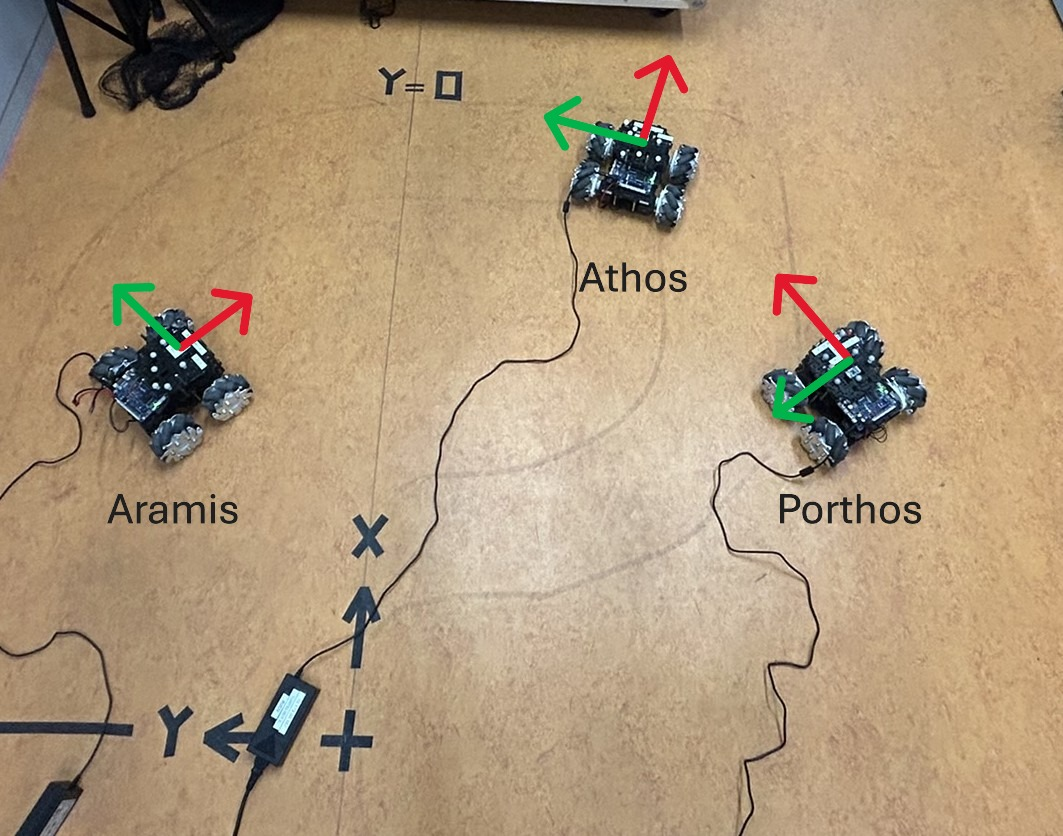
\includegraphics[width=0.7\textwidth]{Annexes/Mecanum_ROS2/tf2/pictures/real_frames.JPG}
    \caption{Démonstration tf2}
    \label{fig:demo_reel}
\end{figure}

\noindent En utilisant tf2, et un outil de visualisation tel que RViz, il est alors possible de visualiser les 3 repères correspondants aux trois robots comme montré ci-dessous.

\begin{figure}[H]
    \centering
    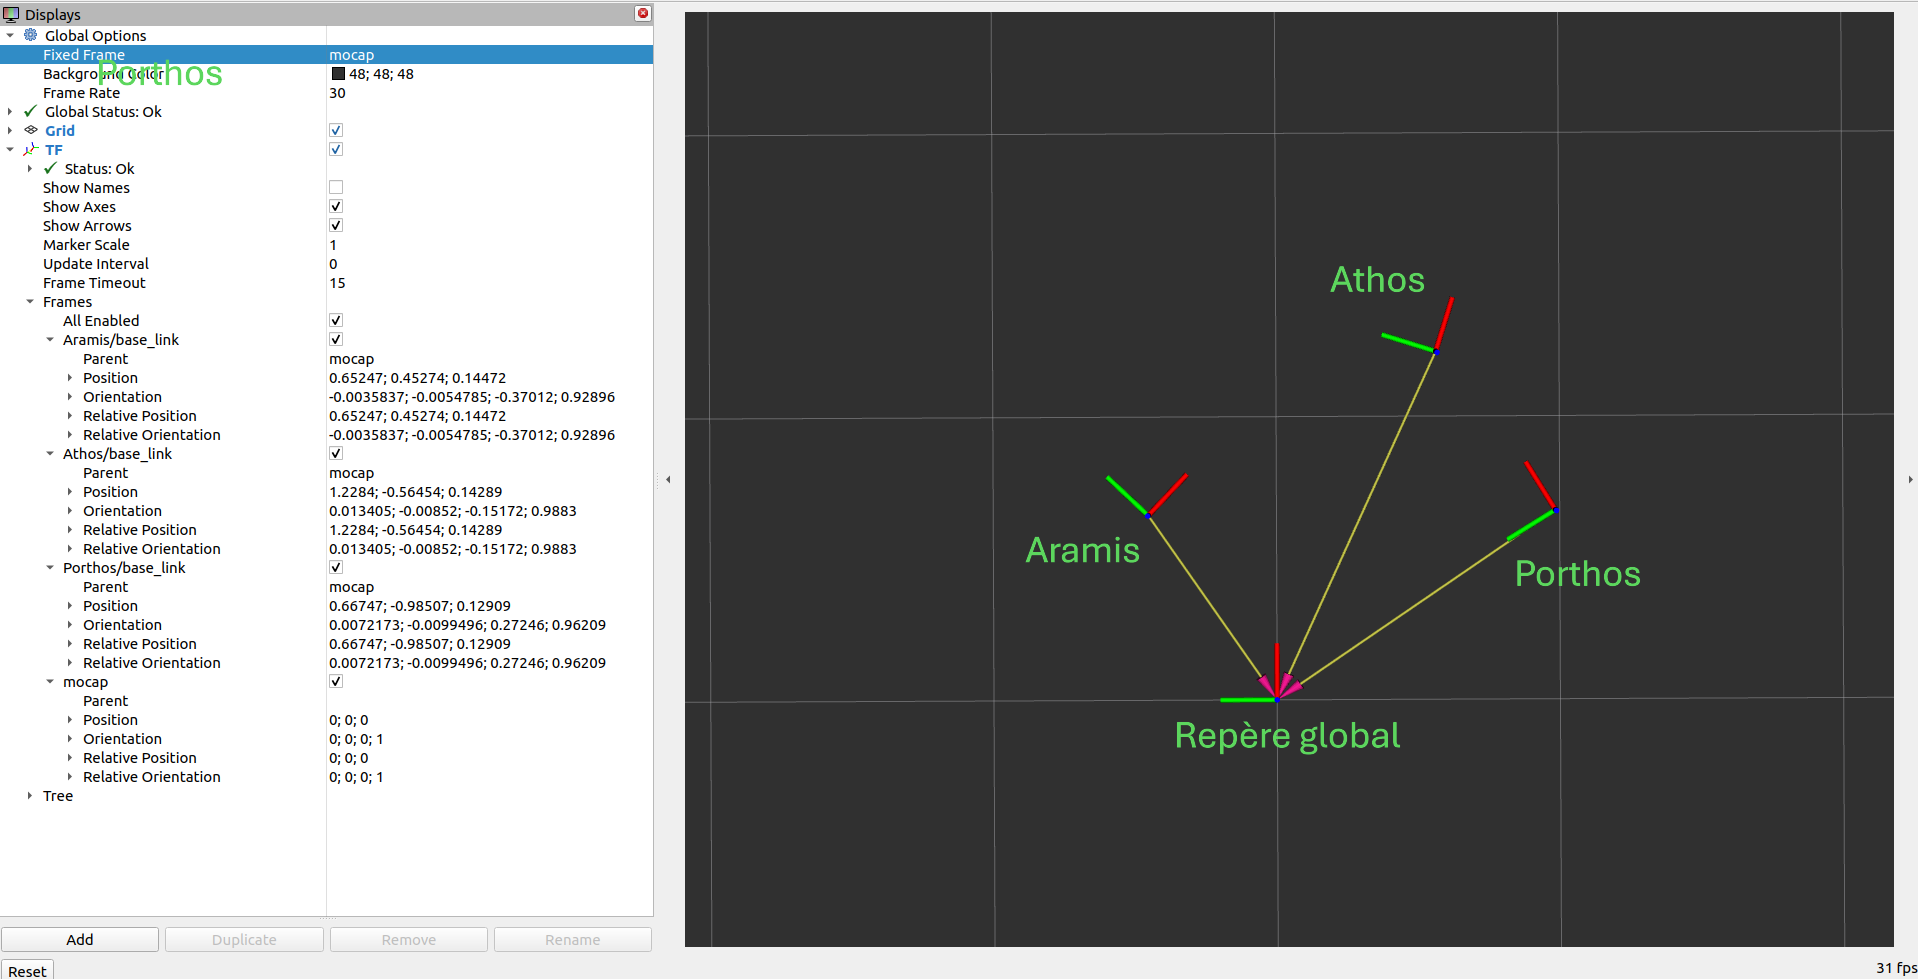
\includegraphics[width=1\textwidth]{Annexes/Mecanum_ROS2/tf2/pictures/rviz.png}
    \caption{Visualisation Rviz}
    \label{fig:rviz}
\end{figure}

\underline{Note : } Pour lancer Rviz, utiliser la commande suivante : 


\begin{lstlisting}[style=commandstyle]
ros2 run rviz2 rviz2 -d $(ros2 pkg prefix --share turtle_tf2_py)/rviz/turtle_rviz.rviz
\end{lstlisting}

